\chapter{Design}

This chapter discusses details of the design of \dolfin{} and is
intended mainly for developers of \dolfin{}.

\section{Linear algebra}

The linear algebra library provides a uniform interface to uBlas
and PETSc linear algebra through a set of wrappers for basic data
structures (matrices and vectors) and solvers, such as Krylov subspace
solvers with preconditioners.

For both sets of wrappers, a common interface is defined by the
classes \texttt{GenericMatrix} and \texttt{GenericVector}. \dolfin{}
provides a number of algorithms, most notably the assembly algorithms,
that work only through the common interface, which means that these
algorithms work for any given representation that implements the
interface specified by \texttt{GenericMatrix} or
\texttt{GenericVector}. A class diagram for the \dolfin{} linear
algebra implementation is given in Figure~\ref{fig:laclasses}.

\begin{figure}[htbp]
  \begin{center}
    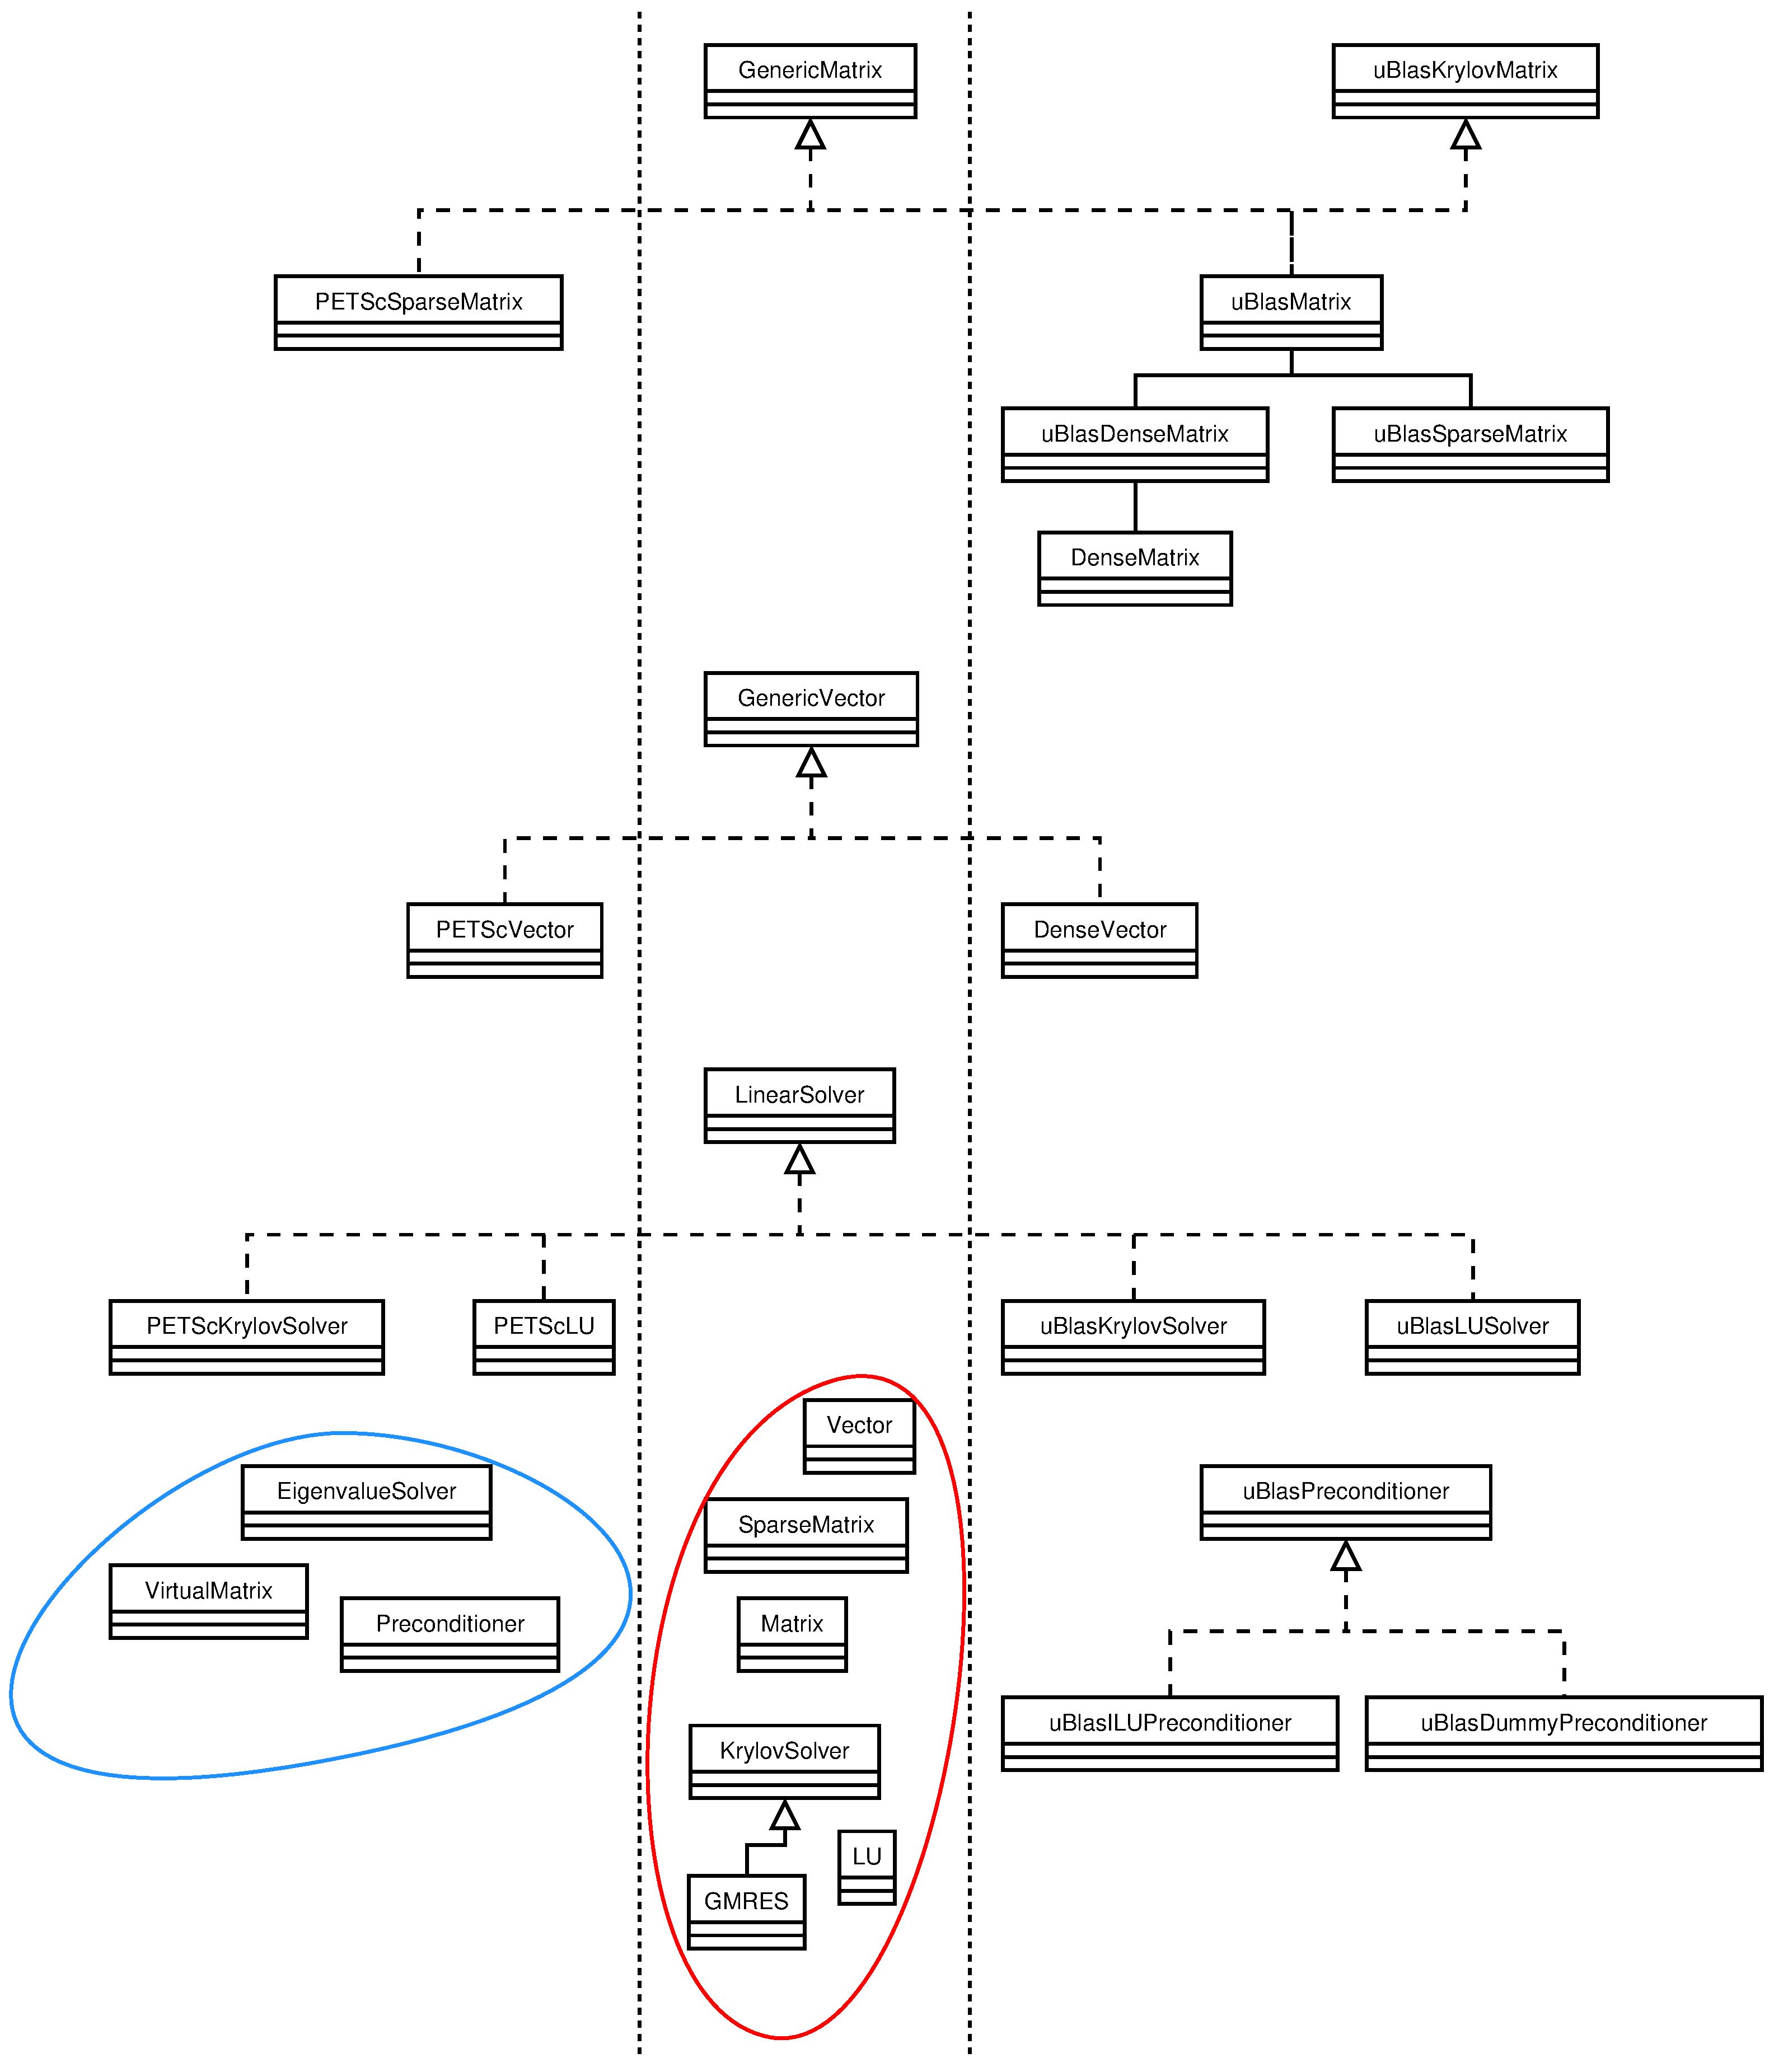
\includegraphics[width=0.95\textwidth]{eps/class-diagram-la.eps}
    \caption{Class diagram of the linear algebra classes in \dolfin{}.}
    \label{fig:laclasses}
  \end{center}
\end{figure}

